\documentclass{beamer}
\usetheme{Montpellier}
%\usepackage[backend=bibtex]{biblatex}
%\bibliography{presentation}
\usepackage[french]{babel}
\usepackage{float}
\usepackage{tikz}
\usepackage{algorithm2e}
\usepackage{graphics}
\usepackage{amsthm}
\usepackage{amsmath}
\usepackage{algpseudocode}
\usepackage{ulem}
\renewcommand{\thefootnote}{\fnsymbol{footnote}}
\newcommand\redout{\bgroup\markoverwith
{\textcolor{red}{\rule[0.5ex]{2pt}{0.8pt}}}\ULon}






\setbeamertemplate{section in toc}{%
  {\inserttocsectionnumber.}~\inserttocsection}
\setbeamercolor{subsection in toc}{bg=white,fg=structure}
\setbeamertemplate{subsection in toc}{%
  \hspace{1.2em}{\rule[0.3ex]{3pt}{3pt}}~\inserttocsubsection\par}


\AtBeginSection[]
{
  \begin{frame}
  \frametitle{Table   de mati\`eres}
  \tableofcontents[currentsection]
  \end{frame}
}


\newcommand{\A}{\mathcal{A}}
\newcommand{\B}{\mathcal{B}}
\newcommand{\D}{\mathcal{D}}
\newcommand{\G}{\mathbb{G}}
\newcommand{\Z}{\mathbb{Z}}
\newcommand{\PR}{\operatorname{Pr}}
\newcommand{\PP}{\mathsf{P}}  
\newcommand{\VV}{\mathsf{V}}  
\newcommand{\K}{\mathsf{K}}  
\newcommand{\SIM}{\mathsf{S}}  
\newcommand{\lbl}{\mathsf{lbl}} 
\newcommand{\PPE}{\mathrm{PPE}} 
\newcommand{\SK}{\mathsf{SK}}
\newcommand{\PK}{\mathsf{PK}}
\newcommand{\VK}{\mathsf{VK}}
\newcommand{\SSK}{\mathsf{SSK}}
\newcommand{\SVK}{\mathsf{SVK}}
\newcommand{\sk}{\mathsf{sk}}
\newcommand{\ck}{\mathsf{ck}}
\newcommand{\tk}{\mathsf{tk}}
\newcommand{\msk}{\mathsf{msk}}
\newcommand{\vk}{\mathsf{vk}}
\newcommand{\ovk}{\mathsf{ovk}}
\newcommand{\pk}{\mathsf{pk}}
\newcommand{\opk}{\mathsf{opk}}
\newcommand{\osk}{\mathsf{osk}}
\newcommand{\com}{\mathsf{com}}
\newcommand{\open}{\mathsf{open}}
\newcommand{\True}{\mathsf{True}}
\newcommand{\False}{\mathsf{False}}
\newcommand{\BF}{\mathbf}
\newcommand{\sample}{\stackrel{{\scriptscriptstyle \mkern4mu R}}{\gets}}
\newcommand{\etal}{\textit{el. al.}}
\newcommand{\eg}{\textrm{e.g.} }
\newcommand{\ie}{\textrm{i.e.} }
\newcommand{\wrt}{\textrm{w.r.t.} }
\newcommand{\st}{\textrm{s.t.} }
\newcommand{\resp}{\textrm{resp.} }
\providecommand{\tprod}{{\textstyle\prod}}
\newcommand{\Setup}{{\mathsf{Setup}}}
\newcommand{\KeyGen}{{\mathsf{KeyGen}}}
\newcommand{\Enc}{{\mathsf{Enc}}}
\newcommand{\Dec}{{\mathsf{Dec}}}
\newcommand{\Rerand}{{\mathsf{ReRandom}}}
\newcommand{\Sig}{{\mathsf{Sign}}}
\newcommand{\Verif}{{\mathsf{Verify}}}
\newcommand{\Prove}{{\mathsf{Prove}}}
\newcommand{\Com}{{\mathsf{Commit}}}
\newcommand{\PPP}{\mathsf{PP}}
\newcommand{\Forge}{\mathsf{Forge}}
\newcommand{\Adv}{\mathcal{A}}


\newcommand{\backupbegin}{
   \newcounter{framenumberappendix}
   \setcounter{framenumberappendix}{\value{framenumber}}
}
\newcommand{\backupend}{
   \addtocounter{framenumberappendix}{-\value{framenumber}}
   \addtocounter{framenumber}{\value{framenumberappendix}} 
}


\setbeamertemplate{footline}[frame number]

\title{Pr\'esentation de protocoles cryptographiques}
\author{Chen Qian}

\institute{\'ENS de Rennes, France}

\begin{document}

\selectlanguage{french}

\begin{frame}
  \maketitle
\end{frame}

\begin{section}{Parcours suivi}
  \begin{frame}{Parcours durant le master}
  
  \begin{enumerate}
  \item Master 1: \'Ecole normale sup\'erieure de Rennes/Universit\'e de Rennes 1 (MRI)  
  \item Stage: Universal Witness Signature. \\NTT Tokyo, Japan(Encadrant: Mehdi Tibouchi)
  \item Master 2: \'Ecole normale sup\'erieure de Rennes/Universit\'e de Paris Diderot (MPRI)
  \item Stage: RCCA chiffrement re-randomizable. \\Lip, \'ENS de Lyon(Encadrants: Beno\^it Libert et Fabien Laguillaumie)
  \end{enumerate}
  
\end{frame}
\end{section}

\begin{section}{Introduction}
  \begin{frame}{Signature Cryptographique}
  \begin{figure}
    
\includegraphics[width=.5\textwidth]{./images/signature.jpg}
  \end{figure}
\end{frame}


\begin{frame}{Introduction : Cryptographie}
  Prot\'eger notre vie, outi puissant pour la s\'ecurit\'e :
  \begin{itemize}
  \item Authenticit\'e et int\'egralit\'e (Signature etc.)
  \item Confidentialit\'e (Chiffrement etc.)
  \end{itemize}
\end{frame}


\begin{frame}{Introduction : Signature}
  \begin{figure}
    \tiny
    \begin{centering}
      \begin{tikzpicture}
        \node (E) at (0,0)[minimum width = 1.5 cm, minimum height = 1.5cm]{
\includegraphics[width = 0.1\textwidth]{images/Alice.png}};
        \node (D) at (5,0)[minimum width = 1.5 cm, minimum height = 1.5cm]{
\includegraphics[width = 0.1\textwidth]{images/Bob.png}}; 

        \pause
        
        \node (ke)[text width = 3.5cm, text centered] at (0,1.5){Clef de signature};
        \path (ke) edge [->] (E.north);

        \node (kd) at (5,1.5){Clef de v\'erification};
        \path (kd) edge [->] (D.north);
        
        \pause
        \node (m) at (-2.5,0){Message $m$};
        \path (m) edge [->] (E);

        \pause

        \path (E) edge[->] node[above]{Signature $\sigma$}(D);
        
        \pause
        
        \node (m2) at (5,-1.5){Vrai ou Faux};
        \path (D) edge [->] (m2);
        
      \end{tikzpicture}
    \end{centering}
  \end{figure}
  
  

  \visible<6->{Un sch\'ema de signature $Sig = (KeyGen, Sign, Verify)$.}
  

  \visible<7->{Correction : $(sk, vk) \gets KeyGen(\lambda)$, $Verify(vk, Sign(sk, m)) = Vrai$}
  

\end{frame}


\begin{frame}{Introduction : Chiffrement \`a clef publique}

  Chiffrement asymm\'etrique (Exemple: sch\'ema de chiffrement ElGamal)

  $\G$ un groupe d'ordre premier $p$, $(g, m) \in \G^2$ et $(a,r) \sample \mathbb{Z}_p^2$.  
  \begin{figure}
    \tiny
    \begin{centering}
      \begin{tikzpicture}
        \node (E) at (0,0)[minimum width = 1.5 cm, minimum height = 1.5cm]{
\includegraphics[width = 0.1\textwidth]{images/Alice.png}};
        \node (D) at (5,0)[minimum width = 1.5 cm, minimum height = 1.5cm]{
\includegraphics[width = 0.1\textwidth]{images/Bob.png}}; 

        \pause
        
        \node (ke)[text width = 3.5cm, text centered] at (0,1.5){Clef de chiffrement $\PK = g^a$};
        \path (ke) edge [->] (E.north);

        \node (kd) at (5,1.5){Clef de d\'echiffrement $\SK = a$};
        \path (kd) edge [->] (D.north);
        
        \pause
        \node (m) at (-2.5,0.5){Message $m$};
        \path (m) edge [->] ([yshift = 0.5cm]E.west);
        \node (r) at (-2.5,-0.5){Al\'ea $r$};
        \path (r) edge [->] ([yshift = -0.5cm]E.west);

        \pause

        \path (E) edge[->] node[above]{$C = (C_1, C_2) = \{g^r, m \cdot g^{ar}\}$}(D);
        
        \pause
        
        \node (m2) at (5,-1.5){Message d\'echiffr\'e $m$};
        \path (D) edge [->] (m2);
        
      \end{tikzpicture}
    \end{centering}
  \end{figure}

  \pause
  \visible<5->{{\color{blue} \emph{Correction}: } $Dec(\SK, Enc(\PK, m, r)) = m$}
  \pause
  \visible<6->{{\color{blue} \emph{IND-CPA(Indistinguishable Chosen-Plaintext Attack)}: } $(m_0, m_1, Enc(\PK, m_0, r_0)) \approx_c (m_0, m_1, Enc(\PK, m_1, r_1))$}
  
\end{frame}

\end{section}

\begin{frame}{Table de mati\`eres}
  \tableofcontents
\end{frame}


\begin{section}{Universal Witness Signature(UWS)}
  
  \begin{subsection}{Application de Universal Witness Signature(UWS)}
    \begin{frame}{Signature redactable: Signer un message partiel}
  \begin{figure}[H]

    \begin{tikzpicture}
      
      \node (TopSecret) at (0,0){
\includegraphics[width = 0.3\textwidth]{./images/Top-Secret.jpg}};
      \node (File) [text width = 3cm,draw,thick,minimum width=1.5cm,minimum height=0.75cm] at (0,0) {32 January 2000, Darth Vader had a dinner with master Yoda.};
      \node (SignatureInit) [text width = 3cm,draw,thick,minimum width=1.5cm,minimum height=0.75cm]at (0,-2) {Signature valide du fichier initial};
      \node (File2) [text width = 3cm,draw,thick,minimum width=1.5cm,minimum height=0.75cm] at (6,0) {32 January 2000, Darth Vader had a dinner with \#\#\#\#\#\#\#\#\#.};
      \node (SignatureFinal)[text width = 3cm,draw,thick,minimum width=1.5cm,minimum height=0.75cm] at (6,-2) {Signature valide du nouveau fichier};
      \path (SignatureInit) edge[->]node[above]{sans $msk$} (SignatureFinal);
      
    \end{tikzpicture}

  \end{figure}

\end{frame}


\begin{frame}{Signature propositionnelle: Signer logiquement}
  \begin{itemize}
  \item \'Element \`a signer: Formules du calcul propositionnel.
  \item Propri\'et\'e sp\'eciale de signature propositionnelle : $Delegate(PP, Sig(Prop_A),Prop_A,Prop_B,w_{Prop_A \Rightarrow Prop_B}) = Sig(Prop_B)$
  \end{itemize}

  Example:

  $(``A", \sigma_{A}) \leadsto (``A\wedge B", \sigma_{A\wedge B})$ 
\end{frame}

  \end{subsection}

  \begin{subsection}{Notre Universal Witness Signature}
    \begin{frame}{G\'en\'eralisation des protocoles pr\'ec\'edents}
  \begin{figure}
    \begin{tikzpicture}
      \node (bot)  at (0,0) {$\bot$};
      \node (A) at (-2,-2) {Proposition $A$, $\SK_{A}$};
      \node (B) at (2,-2) {Proposition $B$, $\SK_{B}$};
      \node (C) at (-4, -4) {Proposition $C$, $\SK_{C}$};
      \path (bot) edge [->] (A);
      \path (bot) edge [->] (B);
      \path (A) edge [->] (C);
    \end{tikzpicture}
  \end{figure}
\end{frame}





\begin{frame}{D\'efinition de Universal Witness Signature}
  \begin{block}{D\'efinition}
    Une Universal Witness Signature par rapport \`a un relation pre-order $Ord$ (qui poss\`ede un plus grand element $*$) est une paire d'algorithmes $(Setup, Delegate)$ qui v\'erifie les sp\'ecifications suivantes :
    \begin{itemize}
    \item $Setup(1^\lambda) \to (PP,SK_*)$: G\'en\'erer un param\`etre publique $PP$ et une clef de signature $SK_*$.
    \item $Delegate(PP, SK_A, A, B, w) \to SK_B$: Si $SK_A$ est une clef de signature valide de $A$ et $w$ est un t\'emoin de $B\leq A$, alors l'algorithme retournera $SK_B$, sinon il retournera $\bot$.
    \end{itemize}
  \end{block}
\end{frame}

%\begin{frame}{Remarques}
 %
 % \begin{tabular}{|c|c|c|}
 %   \hline
 %   & Sch\'ema classique de  & Sch\'ema UWS\\
 %   & signature hi\'erarchique & \\
 %   \hline
 %   Identit\'e  & $Id = (id_1, \dots, id_k)$ & $Id = id_k$\\
 %   \hline
 %   Clef de signature &  $SK_{ID}$ & $SK_{ID}$\\
 %   \hline
 %   Message  & $M = (id_1, \dots, id_k, m)$ & $M = m$ \\
 %   \hline
 %   Signature & $\sigma_m$ & $SK_m$\\
 %   \hline
 % \end{tabular}
 %
 % \begin{block}{}
 %   Algorithme de v\'erification :
 %   $$Verify(PP, m, \sigma_m)  =  Delegate(PP,SK_m,m,m, ``\forall x. x\leq x")$$
 % \end{block}
%\end{frame}



\begin{frame}{Contributions}
  \begin{enumerate}
  \item G\'en\'eralisation de plusieurs notions de sch\'ema de signatures.
  \item Premi\`ere construction de signature propositionnelle.
  \end{enumerate}

\end{frame}
  \end{subsection}

\end{section}

\begin{section}{Chiffrement re-randomisable RCCA}

  \begin{subsection}{Introduction du chiffrement asymm\'etrique}
    

\begin{frame}{Chiffrement re-randomizable}

  Exemple: Chiffrement ElGamal
  
  \begin{figure}
    \tiny
    \begin{centering}
      \begin{tikzpicture}
        \node (E) at (0,0)[minimum width = 1.5 cm, minimum height = 1.5cm]{
\includegraphics[width = 0.1\textwidth]{images/Alice.png}};
        \node (D) at (6,0)[minimum width = 1.5 cm, minimum height = 1.5cm]{
\includegraphics[width = 0.1\textwidth]{images/Bob.png}};
        
        \node (ke) at (0,1.5){Clef de chiffrement $\PK = g^a$};
        \path (ke) edge [->] (E.north);
        \node (kd) at (6,1.5){Clef de d\'echiffrement $\SK = a$};
        \path (kd) edge [->] (D.north);
        
        \node (m) at (-2.5,0.5){Message $m$};
        \path (m) edge [->] ([yshift = 0.5cm]E.west);
        \node (r) at (-2.5,-0.5){Al\'ea $r$};
        \path (r) edge [->] ([yshift = -0.5cm]E.west);

        \pause
        \node (M) at (3,0)[minimum width = 1.5 cm, minimum height = 1.5cm]{
\includegraphics[width = 0.1\textwidth]{images/Merlin.jpg}};
        \path (E) edge[->] node[above]{$c$} node[below]{$=\{g^r, m\cdot g^{ar}\}$}(M);
        \path (M) edge [->] node[above]{$c'$} node[below]{$=\{g^{r'}, m \cdot g^{ar'}\}$}(D);
        \node (m3) at (6,-1.5){Message d\'echiffr\'e $m$};
        \path (D) edge [->] (m3);
        
        
      \end{tikzpicture}
    \end{centering}
  \end{figure}

  \pause
  
  \visible<3->{{\color{blue} \emph{Correction}: } $Dec(\SK, Enc(\PK, m, r)) = m$}
  

\end{frame}



%\begin{frame}{Mixnetwork}
%  
%  \begin{figure}
%    \tiny
%    \begin{tikzpicture}
%      \node (People1) at (0,0)[minimum width = 1.5 cm, minimum height = 1.5cm]{
\includegraphics[width = 0.1\textwidth]{images/people.png}};
%      \node (Server1) at (2,0)[minimum width = 1.5 cm, minimum height = 1.5cm]{
\includegraphics[width = 0.1\textwidth]{images/server.png}};
%      \node (Void) at (4,0)[minimum width = 1.5 cm, minimum height = 1.5cm]{\dots};
%      \node (Server2) at (6,0)[minimum width = 1.5 cm, minimum height = 1.5cm]{
\includegraphics[width = 0.1\textwidth]{images/server.png}};
%      \node (People2) at (8,0)[minimum width = 1.5 cm, minimum height = 1.5cm]{
\includegraphics[width = 0.1\textwidth]{images/people.png}};
%      \node (SK) at (6,2) {Decryption key $sk$};
%      \path (SK) edge[->] (Server2);
% 
%      \path ([yshift = 0.5cm] People1.east) edge[->] node[above]{$c_1$} ([yshift = 0.5cm] Server1.west);
%      \path ([yshift = 0cm] People1.east) edge[->] node[above]{$c_2$}([yshift = 0cm] Server1.west);
%      \path ([yshift = -0.5cm] People1.east) edge[->] node[above]{$c_3$}([yshift = -0.5cm] Server1.west);
% 
%      \path ([yshift = 0.5cm] Server1.east) edge[->] ([yshift = 0cm] Void.west);
%      \path ([yshift = 0cm] Server1.east) edge[->] ([yshift = -0.5cm] Void.west);
%      \path ([yshift = -0.5cm] Server1.east) edge[->] ([yshift = 0.5cm] Void.west);
%      
%      \path ([yshift = 0.5cm] Void.east) edge[->] ([yshift = -0.5cm] Server2.west);
%      \path ([yshift = 0cm] Void.east) edge[->] ([yshift = 0.5cm] Server2.west);
%      \path ([yshift = -0.5cm] Void.east) edge[->] ([yshift = 0cm] Server2.west);
%      
%      \path ([yshift = 0.5cm] Server2.east) edge[->] node[above]{$m_1$}([yshift = 0.5cm] People2.west);
%      \path ([yshift = 0cm] Server2.east) edge[->] node[above]{$m_2$}([yshift = 0cm] People2.west);
%      \path ([yshift = -0.5cm] Server2.east) edge[->] node[above]{$m_3$}([yshift = -0.5cm] People2.west);
%    \end{tikzpicture}
%  \end{figure}
%\end{frame}

\begin{frame}{Syst\`eme de vote sans re\c{c}u}

  Exemple: ElGamal

  \begin{figure}
    \tiny
    \begin{tikzpicture}
      \node (A) at (0,0)[minimum width = 1.5 cm]{
\includegraphics[width=0.1\textwidth]{images/Alice.png}};
      \node (Adv) at (0,3)[minimum width = 1.5 cm]{
\includegraphics[width=0.1\textwidth]{images/Eve.png}};
      \node (Gov) at (6,0)[minimum width = 1.5 cm]{
\includegraphics[width=0.1\textwidth]{images/government.png}};
      \path (A) edge[->] node[above]{Vote : $c = \{g^r, m\cdot g^{ar}\}$} (Gov);
      \path ([xshift = -0.25cm]Adv.south) edge[->] node[below,sloped]{\tiny Donne-moi une preuve!}([xshift = -0.25cm]A.north);
      \path ([xshift = 0.25cm]A.north) edge[->] node[below,sloped]{\tiny La preuve est $r$.}([xshift = 0.25cm]Adv.south);
      \path (Gov) edge[->] node[above]{Corrompu}(Adv);
    \end{tikzpicture}
   \end{figure}
\end{frame}




\begin{frame}{Syst\`eme de vote sans re\c{c}u}
  \begin{figure}
    \tiny
    \begin{tikzpicture}
      \node (A) at (0,0)[minimum width = 1.5 cm]{
\includegraphics[width=0.1\textwidth]{images/Alice.png}};
      \node (Adv) at (0,3)[minimum width = 1.5 cm]{
\includegraphics[width=0.1\textwidth]{images/Eve.png}};
      \node (Server) at (3,0)[minimum width = 1.5 cm]{
\includegraphics[width=0.1\textwidth]{images/server.png}};
      \node (Gov) at (6,0)[minimum width = 1.5 cm]{
\includegraphics[width=0.1\textwidth]{images/government.png}};
      \path (A) edge[->] node[above]{Vote $\{g^r, g^{ar}\}$} (Server);
      \path ([xshift = -0.25cm]Adv.south) edge[->] node[below,sloped]{\tiny Donne-moi une preuve!}([xshift = -0.25cm]A.north);
      \path ([xshift = 0.25cm]A.north) edge[->] node[below,sloped]{\tiny Je ne peux pas!}([xshift = 0.25cm]Adv.south);
      \path (Server) edge[->]node[above]{Votes re-randomiz\'es} node[below]{$\{g^{r'}, g^{ar'}\}$} (Gov);
      \path (Gov) edge[->] node[above]{Corrompu}(Adv);
    \end{tikzpicture}
   \end{figure}
\end{frame}


\begin{frame}{Indistinguishable Chosen-Ciphertext Attack (IND-CCA) et Replayable Chosen-Ciphertext Attack (RCCA)}
  \alt<2->{RCCA}{IND-CCA}
  %  \begin{figure}
  %    \tiny
  %    \begin{centering}
  % 
  %      \begin{tikzpicture}
  % 
  %        \node (A) at (3,0)[draw, thick, minimum width = 1.5 cm, minimum height = 3cm]{
\includegraphics[width=0.1\textwidth]{images/Eve.png}};
  %        \node (D) at (6,0)[draw, thick, minimum width = 1.5 cm, minimum height = 3cm]{
\includegraphics[width = 0.05\textwidth]{images/Bob.png}};
  %        \node (E) at (0,0)[draw, thick, minimum width = 1 cm, minimum height = 1cm]{
\includegraphics[width = 0.05\textwidth]{images/Alice.png}};
  %        
  %        
  %        \node (mb) at (-2,0.25){$b$};
  %        \path (mb) edge [->] ([yshift = 0.25cm]E.west);
  %        \node (r) at (-2,-0.25){$r$};
  %        \path (r) edge [->] ([yshift = -0.25cm]E.west);
  % 
  %        \path (E) edge[->] node[above]{$c^* = Enc(m_b; r)$}(A);
  % 
  %        \path ([yshift = 1.25cm]A.east) edge[->] node[above]{$\{c_i\}$}([yshift = 1.25cm]D.west);
  %        \path ([yshift = 0.75cm]A.east) edge[<-] node[above]{$\{m_i\}$}([yshift = 0.75cm]D.west);
  %        
  %        \path ([yshift = -0.75cm]A.east) edge[->] node[above]{\alt<2>{Cond\footnote{$Dec(k_d, \{c_j\}) \not \in \{m_0,m_1\}$}}{$\{c_j\}\neq c^*$}}([yshift = -0.75cm]D.west);
  %        \path ([yshift = -1.25cm]A.east) edge[<-] node[above]{$\{m_j\}$}([yshift = -1.25cm]D.west);
  %        
  %        
  %        \node (b') at (1,-1){$b'$};
  %        \path ([yshift= -1cm]A.west) edge[->] (b');
  % 
  %        
  %        \node (ke) at (3,2.5){$k_e$};
  %        \path (ke) edge[->](A);
  %        \node (kd) at (6,2.5){$k_d$};
  %        \path (kd) edge[->](D);
  %        
  %        \node (m0) at (1.5,1.25){$m_0$};
  %        \path ([yshift = 1.25cm]A.west) edge[->] (m0);
  %        \node (m1) at (1.5,0.75){$m_1$};
  %        \path ([yshift = 0.75cm]A.west) edge[->] (m1);
  % 
  % 
  %        \node (def)[align=left] at (-3,2){$b\in\{0,1\}$, $r$ random \\ $|r| = |m_0| = |m_1|$ \\ $i \in Query1$ \\ $j \in Query2$};
  %      \end{tikzpicture}
  % 
  %    \end{centering}
  %  \end{figure}

  \begin{figure}
    \begin{tikzpicture}
      \node(A)[draw, thick, text width = 1.7cm, minimum height = 3cm] at (0,0) {Adversaire};
      \node(C)[draw, thick, text width = 1.7cm, minimum height = 3cm] at (4,0) {Challenger};
      \node(D)[draw, thick, text width = 2.1cm, minimum height = 3cm] at (-4,0) {Oracle de d\'echiffrement};
      
      \path([yshift = 1.4cm]A.east) edge[<-] node[above]{$\PK$} ([yshift = 1.4cm]C.west);
      \path([yshift = 1cm]D.east) edge[<-] node[above]{$C_i$} ([yshift = 1cm]A.west);
      \path([yshift = 0.6cm]D.east) edge[->] node[above]{$m_i$} ([yshift = 0.6cm]A.west);
      \path([yshift = 0.2cm]A.east) edge[->] node[above]{$m_0, m_1$} ([yshift = 0.2cm]C.west);
      
      \path([yshift = -0.3cm]A.east) edge[<-] node[above]{$C_b$}([yshift = -0.3cm]C.west);
      \path([yshift = -0.6cm]D.east) edge[<-] node[above]{\alt<2>{Cond\footnote{$Dec(k_d, \{C_j\}) \not \in \{m_0,m_1\}$}}{$\{C_j\}\neq C_b$}} ([yshift = -0.6cm]A.west);
      \path([yshift = -1cm]D.east) edge[->] node[above]{$m_i$} ([yshift = -1cm]A.west);
      
      \path([yshift = -1.4cm]A.east) edge[->] node[above]{$b'$}([yshift = -1.4cm]C.west);
    \end{tikzpicture}
    
  \end{figure}

  {\color{blue} Advantage:} $Adv(\Adv) = |\PR[b = b'] - \frac{1}{2}|$.
\end{frame}

  \end{subsection}
  
  \begin{subsection}{Nos Contributions}
    \begin{frame}{Nos contributions}
  \setbeamercolor{normal text}{fg=gray,bg=}
  \setbeamercolor{alerted text}{fg=black,bg=}
  \usebeamercolor{normal text}

  \begin{enumerate}
  \item\alert<+>{ Evaluation de l'efficacit\'e du sch\'ema de chiffrement mall\'eable [Chase \etal~2012] $93\times\G$ sous l'hypoth\`ese DLIN ou $49\times\G +20 \times\hat{\G}$ sous l'hypoth\`ese SXDH.}
  \item\alert<+>{ Construction d'un sch\'ema de chiffrement publiquement v\'erifiable qui garde la structure de groupe $16\times\G + 11\times\hat{\G}$ contre $321\times\G$ [Abe \etal~2013].}
  \item\alert<+>{ Construction de notre propre sch\'ema de chiffrement re-randomizable RCCA $29 \times\G + 20 \times\hat{\G}$.}
  \end{enumerate}
\end{frame}

  \end{subsection}

\end{section}


\begin{section}{Th\`ese}
  \begin{frame}{Challenge de l'ordinateur pour la cryptographie}

  \begin{figure}[H]
    \centering
    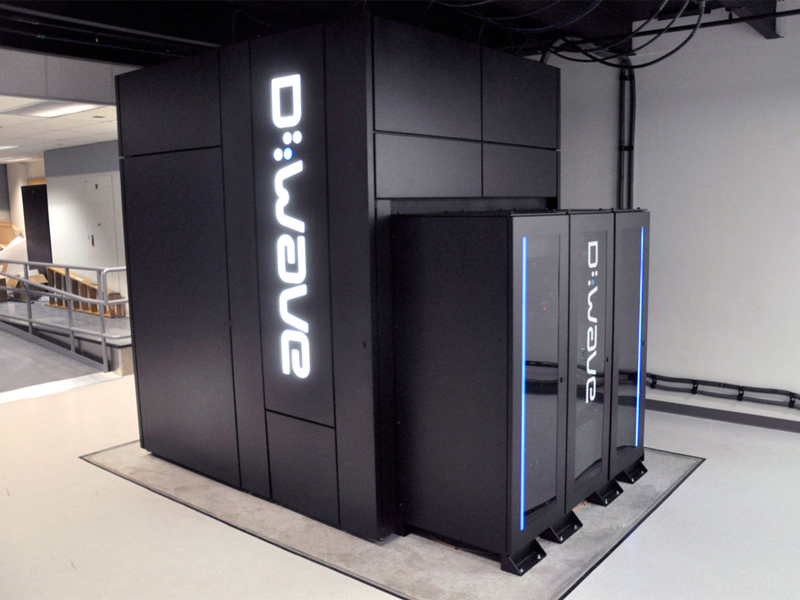
\includegraphics[width= .2\textwidth]{./images/quantum.jpg}
    \caption{``faux'' Ordinateur quantique D-wave}
  \end{figure}
  
  Cryptographie post-quantique candidates :

  \begin{itemize}
  \item Multi-variants
  \item Bas\'e sur les codes
  \item Bas\'e sur les r\'eseaux euclidiens (le seul qui peut fournir des arguments convaincants)
  \end{itemize}

\end{frame}


\begin{frame}{Th\`ese}
  \begin{itemize}
  \item Doctorant dans l'\'equipe EMSEC de l'IRISA \`a \\Universit\'e de Rennes 1. (Depuis 1er septembre 2016)
  \item Encadrant de th\`ese: Pierre-Alain Fouque, Adeline Langlois et Beno\^it Libert
  \item Sujet: Protocoles Cryptographique Post-quantique bas\'e sur le r\'eseau euclidien.
  \end{itemize}
\end{frame}

\end{section}


%\backupbegin
%\begin{frame}[plain, allowframebreaks,noframenumbering]
%    \frametitle{References}
%    \bibliographystyle{apalike}
%    {\tiny \bibliography{presentation}}
%\end{frame}
%\backupend

\end{document}


